\documentclass[lettersize,journal,english]{IEEEtran}
\usepackage[T1]{fontenc}
\usepackage[utf8]{inputenc}
\usepackage{amsmath,amsfonts,amssymb}
\usepackage{algorithmic}
\usepackage{algorithm}
\usepackage{array}
\usepackage[caption=false,font=normalsize,labelfont=sf,textfont=sf]{subfig}
\usepackage{textcomp}
\usepackage{stfloats}
\usepackage{url}
\usepackage{verbatim}
\usepackage{graphicx}
\usepackage{cite}
\usepackage{booktabs}
\usepackage{units}
\usepackage[unicode=true,pdfusetitle,
 bookmarks=true,bookmarksnumbered=false,bookmarksopen=false,
 breaklinks=false,pdfborder={0 0 0},pdfborderstyle={},backref=false,colorlinks=true]{hyperref}
\hypersetup{
 urlcolor=blue, linkcolor=black}
\usepackage[acronym]{glossaries}
\hyphenation{op-tical net-works semi-conduc-tor IEEE-Xplore}

\global\long\def\BDsites{\textsf{BD\_sites}}

\title{Adaptative neigbouring methods applied to telephonic base stations}
\author{Paul MÉHAUD, Brendan SÉVELLEC}

\makeglossaries

\setglossarypreamble{All definitions are from \href{https://www.dictionary.com/}{Dictionnary.com}}

\newglossaryentry{base station}
{
    name=base station,
    description={A fixed transmitter that forms part of an otherwise mobile radio network}
}

\newglossaryentry{convHull}
{
    name=convex hull,
    description={The smallest convex set containing a given set}
}



\newacronym{arcep}{ARCEP}{French Regulatory Authority for Electronic Communications and Posts}
\newacronym{anfr}{ANFR}{French National Frequency Agency}
\newacronym{bs}{BS}{\Gls{base station}}
\newacronym{dbscan}{DBScan}{Density-Based Spatial Clustering of Applications with Noise}
\newacronym{hdbscan}{HDBScan}{Hierarchical Density-Based Spatial Clustering of Applications with Noise}

\usepackage[english,french]{babel}

\begin{document}
\selectlanguage{english}
\maketitle

\begin{abstract}
  The field of telecommunication represents a gigantic mine of information, the smartphone penetration rate being 69\%
  in 2023 in the world, and 97\% in France. Therefore, the collected datas represent a big opportunity for telecommunication
  companies to predict their customers behaviour for internal or marketing purposes. Thus, it is primordial for these companies
  to be able to determinate if a user is moving. For that, it is necessary to understand the neighbouring relationships between the 
  telephonic base stations. This article aims at comparing different method, ellaborated in order to adaptively detect these
  relationship between telephonic base stations given their geographical positions.
\end{abstract}

\section{Introduction}
    \IEEEPARstart{T}{his} article is the continuation of the work done by Delphine Paquiry in this paper \cite{art_del_paq}.
    It aims at discovering the neighbouring relationships between base stations from their geographical positions, using a 
    measure of the density of base station.

    For that, it is necessary to describe and analyse the databases that have been used during the research, then to present 
    the different approaches that always consist of these steps : establish a first neighbouring graph, compute the base station 
    densities and filter this graph with different criteria using this information. The final step is to present the results
    of the different approaches and conclude.
\section{Related works}

\section{Databases}
    Several databases have been used in order to test the different aspects of the methods. However, one of
    them is directly necessary to the method itself.

    \subsection{Main database}

    This database \cite{main_database} contains all the information needed to the application of the method. It is from
    \acrfull{arcep}, which is an independent French administrative authority responsible for regulating electronic and postal communications and press distribution.

    The fields that are being used here are described in Table~\ref{table:data_columns}.

\begin{table}[!b]
    \centering
    \caption{Description of the dataset}
    \label{table:data_columns}
    \begin{tabular}{ll}
        \toprule
        \textbf{Column} & \textbf{Description} \\
        \cmidrule(lr){1-2}
        \textsl{BS\_anfr\_id} & \acrshort{anfr} \acrshort{bs} ID \\ 
        \textsl{x, y, latitude, longitude} & Base station coordinates \\ 
        \textsl{nom\_reg, nom\_dep, nom\_com} & Additional location information \\  
        \textsl{site\_2g, 3g, 4g, 5g} & Technology used by the \acrshort{bs} \\ 
        \bottomrule
    \end{tabular}
\end{table}

\section{Finding potential neighbours}
\noindent When we are looking for neighbours, we need, at first, a list of potential neighbours for each \acrfull{bs}.
For that, we will construct a neigbouring graph $G = (P, U)$ (each base station that are considered neighbors are
connected by an edge) where $P$ is the set of all base stations. 
Here are the different methods we can build this graph with:

\subsection{$k$-NN graph}
\noindent The most intuitive method is to connect each \acrshort{bs} to its $k$ nearest neighbours, where $k \in \mathbb{N}^*$ 
is a parameter to be fixed. 

However, this method can be criticized, because it always finds $k$ neighbor to each base stations, no matter the reality of the 
data.

\subsection{Delaunay triangulation}
\noindent The Delaunay triangulation is named after Boris DELAUNAY for his work on it from 1934 \cite{art_delaunay}.

A Delaunay triangulation of a set of points in the plane subdivides their \gls{convHull} into triangles whose circumcircles 
do not contain any of the points. You can find an illustration of this method in Figure~\ref{fig:del_tri}.

A Voronoi diagram is a tessellation pattern in which $n$ points scattered on a plane subdivides in 
exactly $n$ cells enclosing a portion of the plane that is closest to each point. 

The Delaunay triangulation is the pendant of the Voronoi diagram in the sense that two points are connected in the
Delaunay triangulation if their associated cells share an edge in the Voronoi diagram. 

Therefore, another approach, consists in computing a Delaunay triangulation and build a neighouring graph $G = (P, U)$ where $U$ 
is composed of every edge of $D(P)$. Which is equivalent to consider two base station as potential neighbors if their associated
cells are touching each other in the Voronoi diagram.

This method has already been used in articles in the past \cite{delaunay_neighbor}.


\begin{figure}[!t]
    \centering
    \boxed{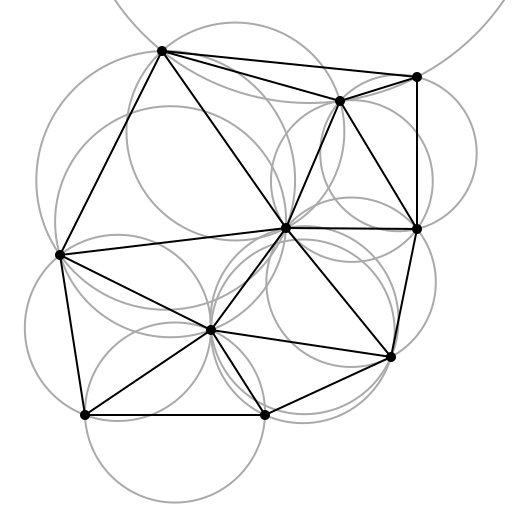
\includegraphics[width=1.25in]{images/illus_graphs/Delaunay_circumcircles_vectorial.png}}
    \boxed{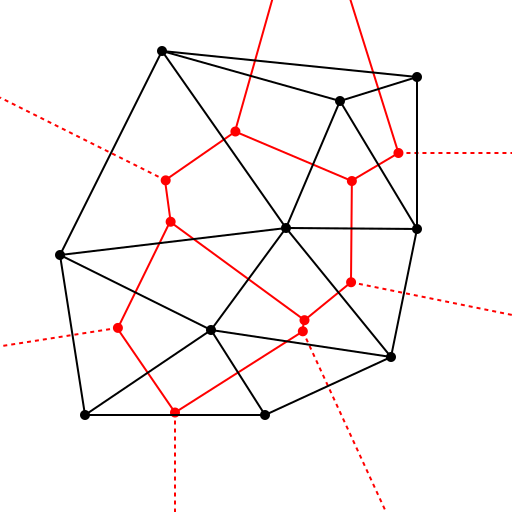
\includegraphics[width=1.25in]{images/illus_graphs/Delaunay_Voronoi.png}}
    \caption{Example of a Delaunay triangulation (in black) and Voronoi tessellation (in red)}
    \label{fig:del_tri}
\end{figure}

\subsection{Gabriel graph}
\noindent The Gabriel graph is a subgraph of a Delaunay triangulation. Thus, if the Delaunay triangulation is given, it can be found in a linear time. 

Gabriel graphs are named after K. Ruben Gabriel, who introduced them in a paper with Robert R. Sokal in 1969 \cite{10.2307/2412323}.

Formally, it is the graph $G = (P, U)$ in which any two distinct points $p, q \in P$ are adjacent precisely when the closed disc having $pq$ as a diameter contains no other points.

Basically, the interset of this method, compared to the Delaunay triangulation, is that it is adding a first level of filtration to suppress some neighbouring connexions.

\section{Finding the real neighbours}

\noindent Each of the precedent methods gives us a list of potential neighbours for each \acrshort{bs}. However, we know that some of this neighbouring connexions are wrong,
either because of the neighboring graph construction method or physical specificities linked to the base stations themselves.

Thus, we need to find methods to detetect and erase these bad connexions.

The main innovation of our work compared to this one \cite{art_del_paq} is to take in account the difference of \acrshort{bs}'s density.

\subsection{Measurement of \acrshort{bs} density}
\noindent To simplify the explanation, and because it is related, we will assume that solving this problem is equivalent to finding the \acrshort{bs} situated in \og cities\fg{}.

\subsubsection{\acrshort{dbscan}}
When thinking of density-based clustering, one of the first methods that comes in mind is probably \acrshort{dbscan}.
It is really powerful because we only have two parameters to modify.

Despite the efficiency of this method, it is not the best adapted to our problem because it's only giving us if a \acrshort{bs} is considered in a city or not.
We wanted a more continuous method.

\subsubsection{\acrshort{hdbscan}}

\subsubsection{$3$-NN mean distance}
To classify each base station we need a method.

For each base station the mean distance to its three nearest neighbours is calculated (we will call this value $\gamma_i$, in $\unit{km}$), thus making it possible to classify each base station into four different categories listed in Table~\ref{table:crit_summary}.

To make this method working properly, only \acrshort{bs} from one provider have to be kept into the calculation process.
Moreover, this values are working well on France but it is not proven that it can work in another country. If someone uses this methods, values could be modified.

\subsection{Filtering criteria}

\begin{table}[!b]
    \centering
    \caption{Summary of criteria values}
    \label{table:crit_summary}
    \begin{tabular}{clcc}
        \toprule
        \textbf{$\gamma_i$} & \textbf{Description} & \textbf{\emph{max\_distance}} & \textbf{\emph{min\_angle}} \\
        \cmidrule(lr){1-4}
        $\left[0, 1\right]$ & city center & $\unit[2]{km}$ & $5^\circ$ \\
        $\left]1, 2\right]$ & urban area & $\unit[5]{km}$ & $10^\circ$ \\
        $\left]2, 4\right]$ & extra-urban area & $\unit[10]{km}$ & $15^\circ$ \\
        $\left]4, \infty\right[$ & courntryside & $\unit[15]{km}$ & $20^\circ$ \\
        \bottomrule
    \end{tabular}
\end{table}

\begin{figure}[!t]
    \centering
    \boxed{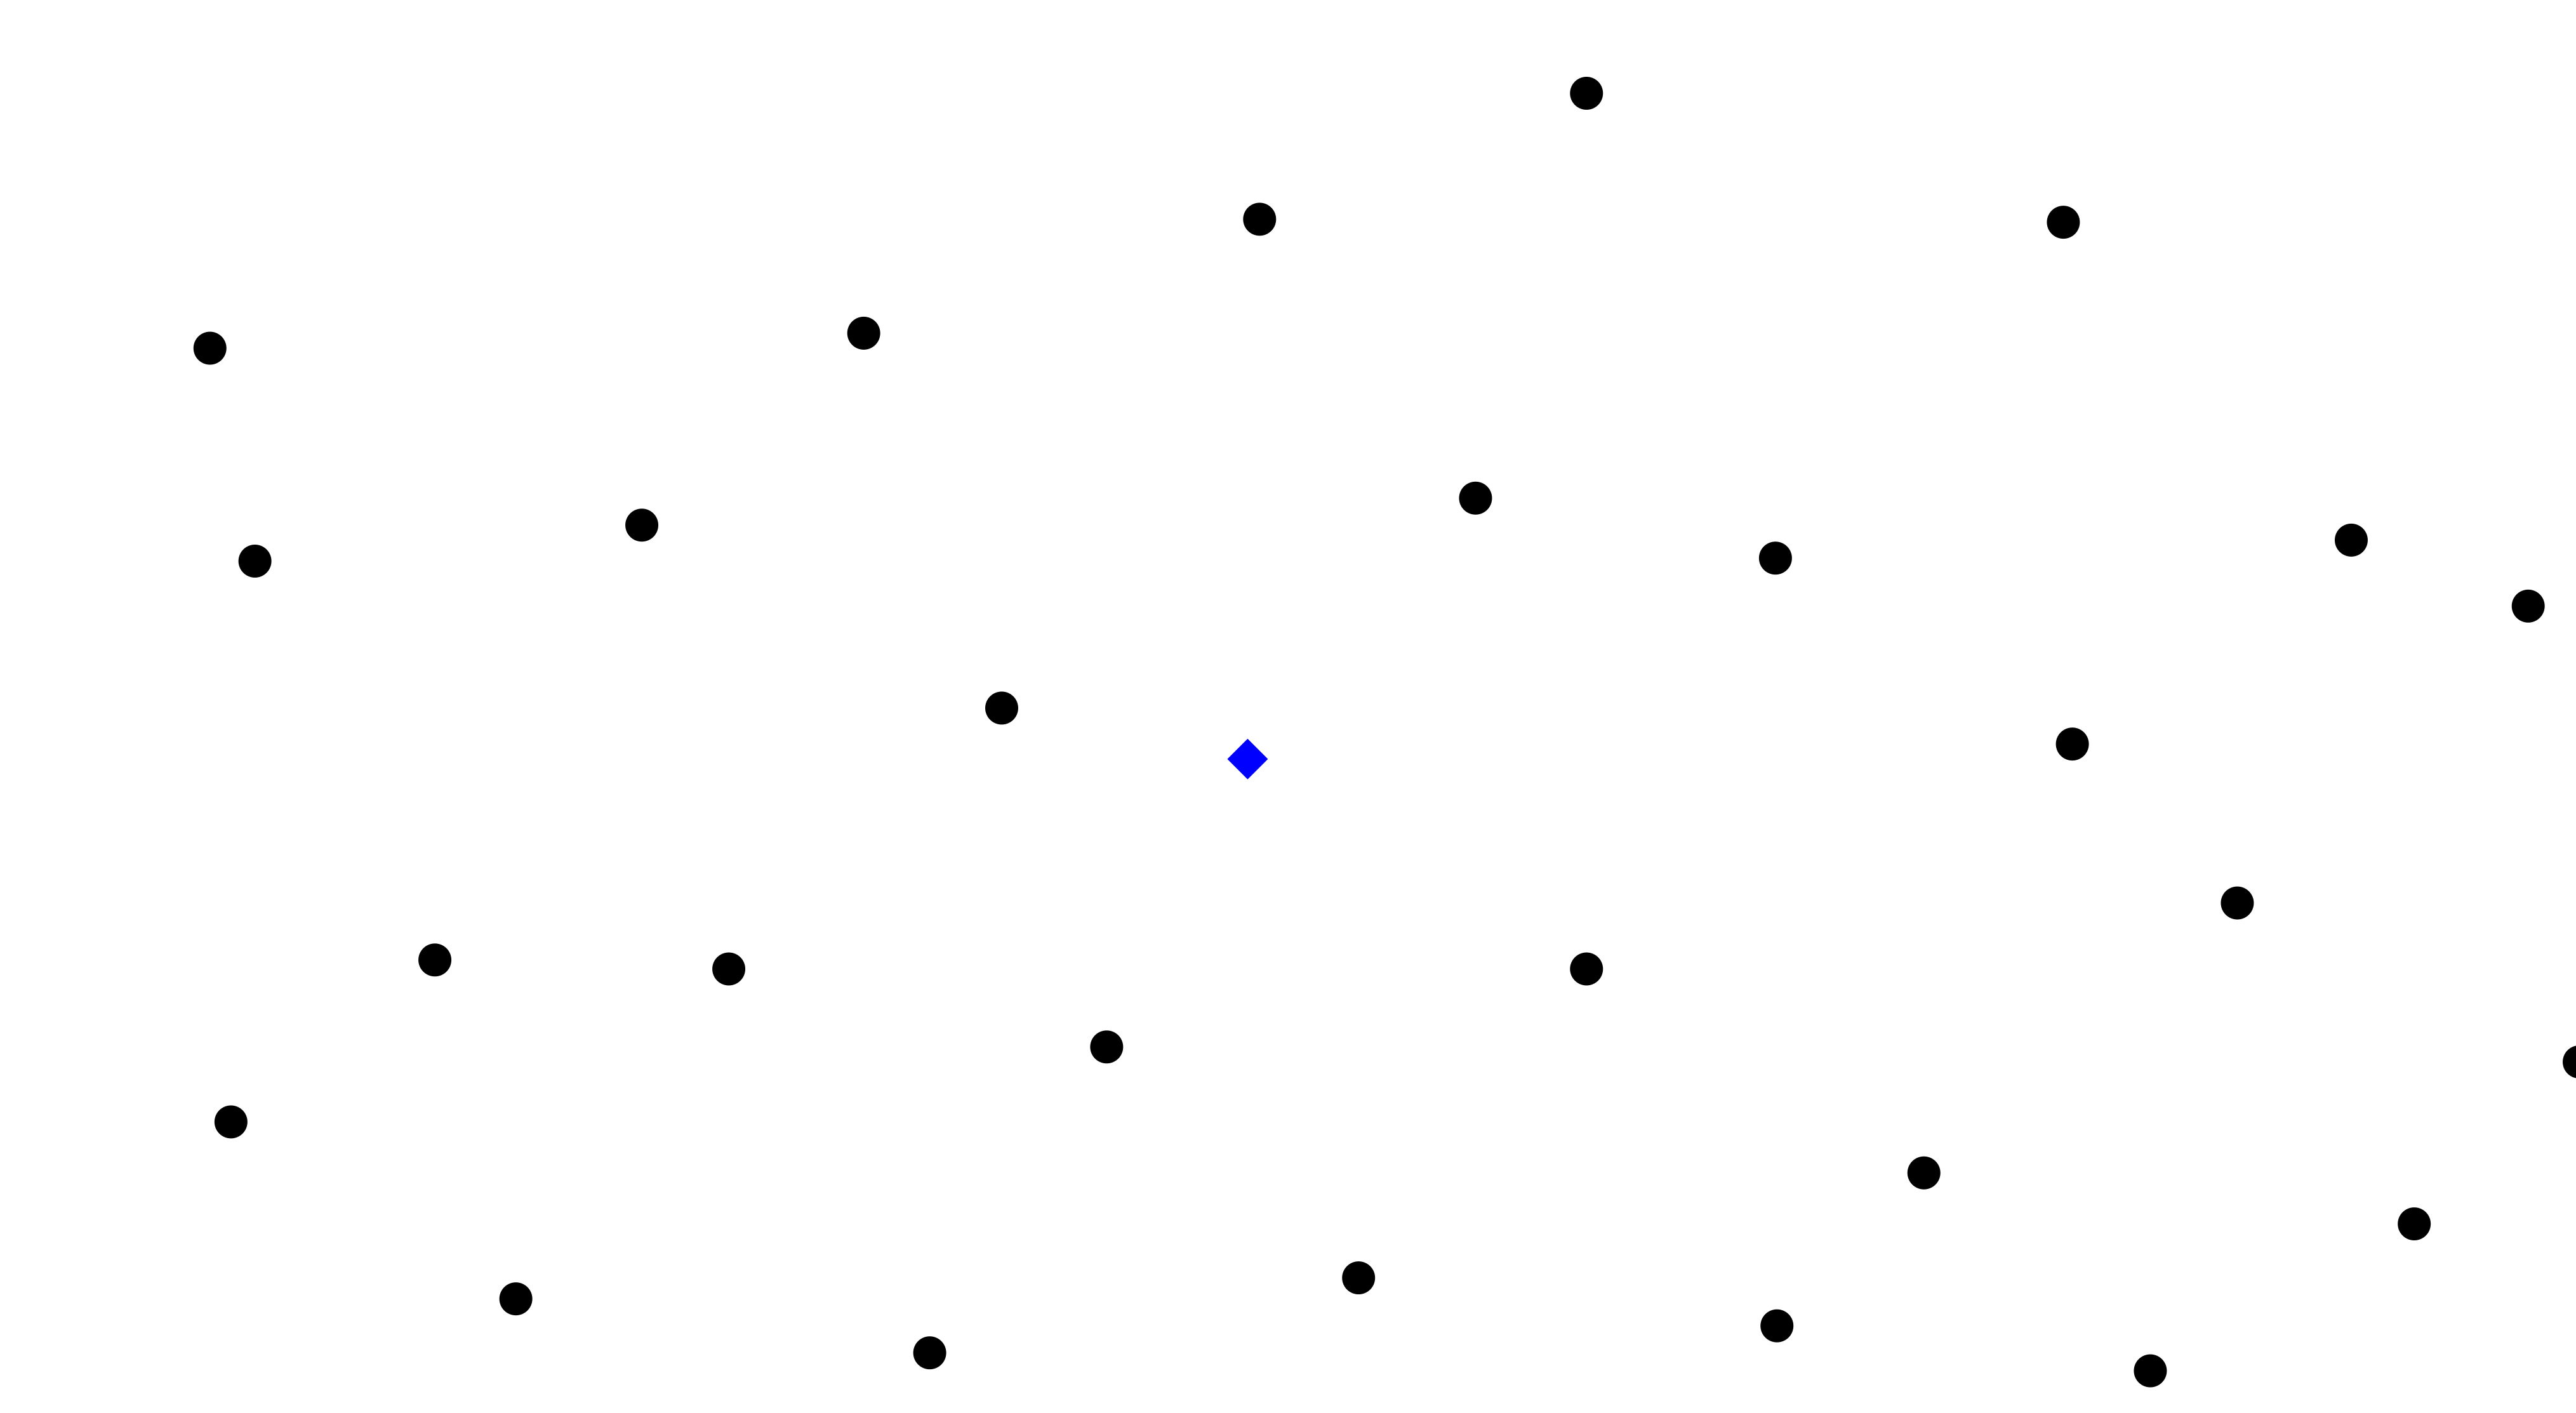
\includegraphics[width=2.5in]{images/illus_crit/points.png}}
    \caption{Example of a Delaunay triangulation}
    \label{fig:crit_pts}
\end{figure}

\begin{figure}[!b]
    \centering
    \boxed{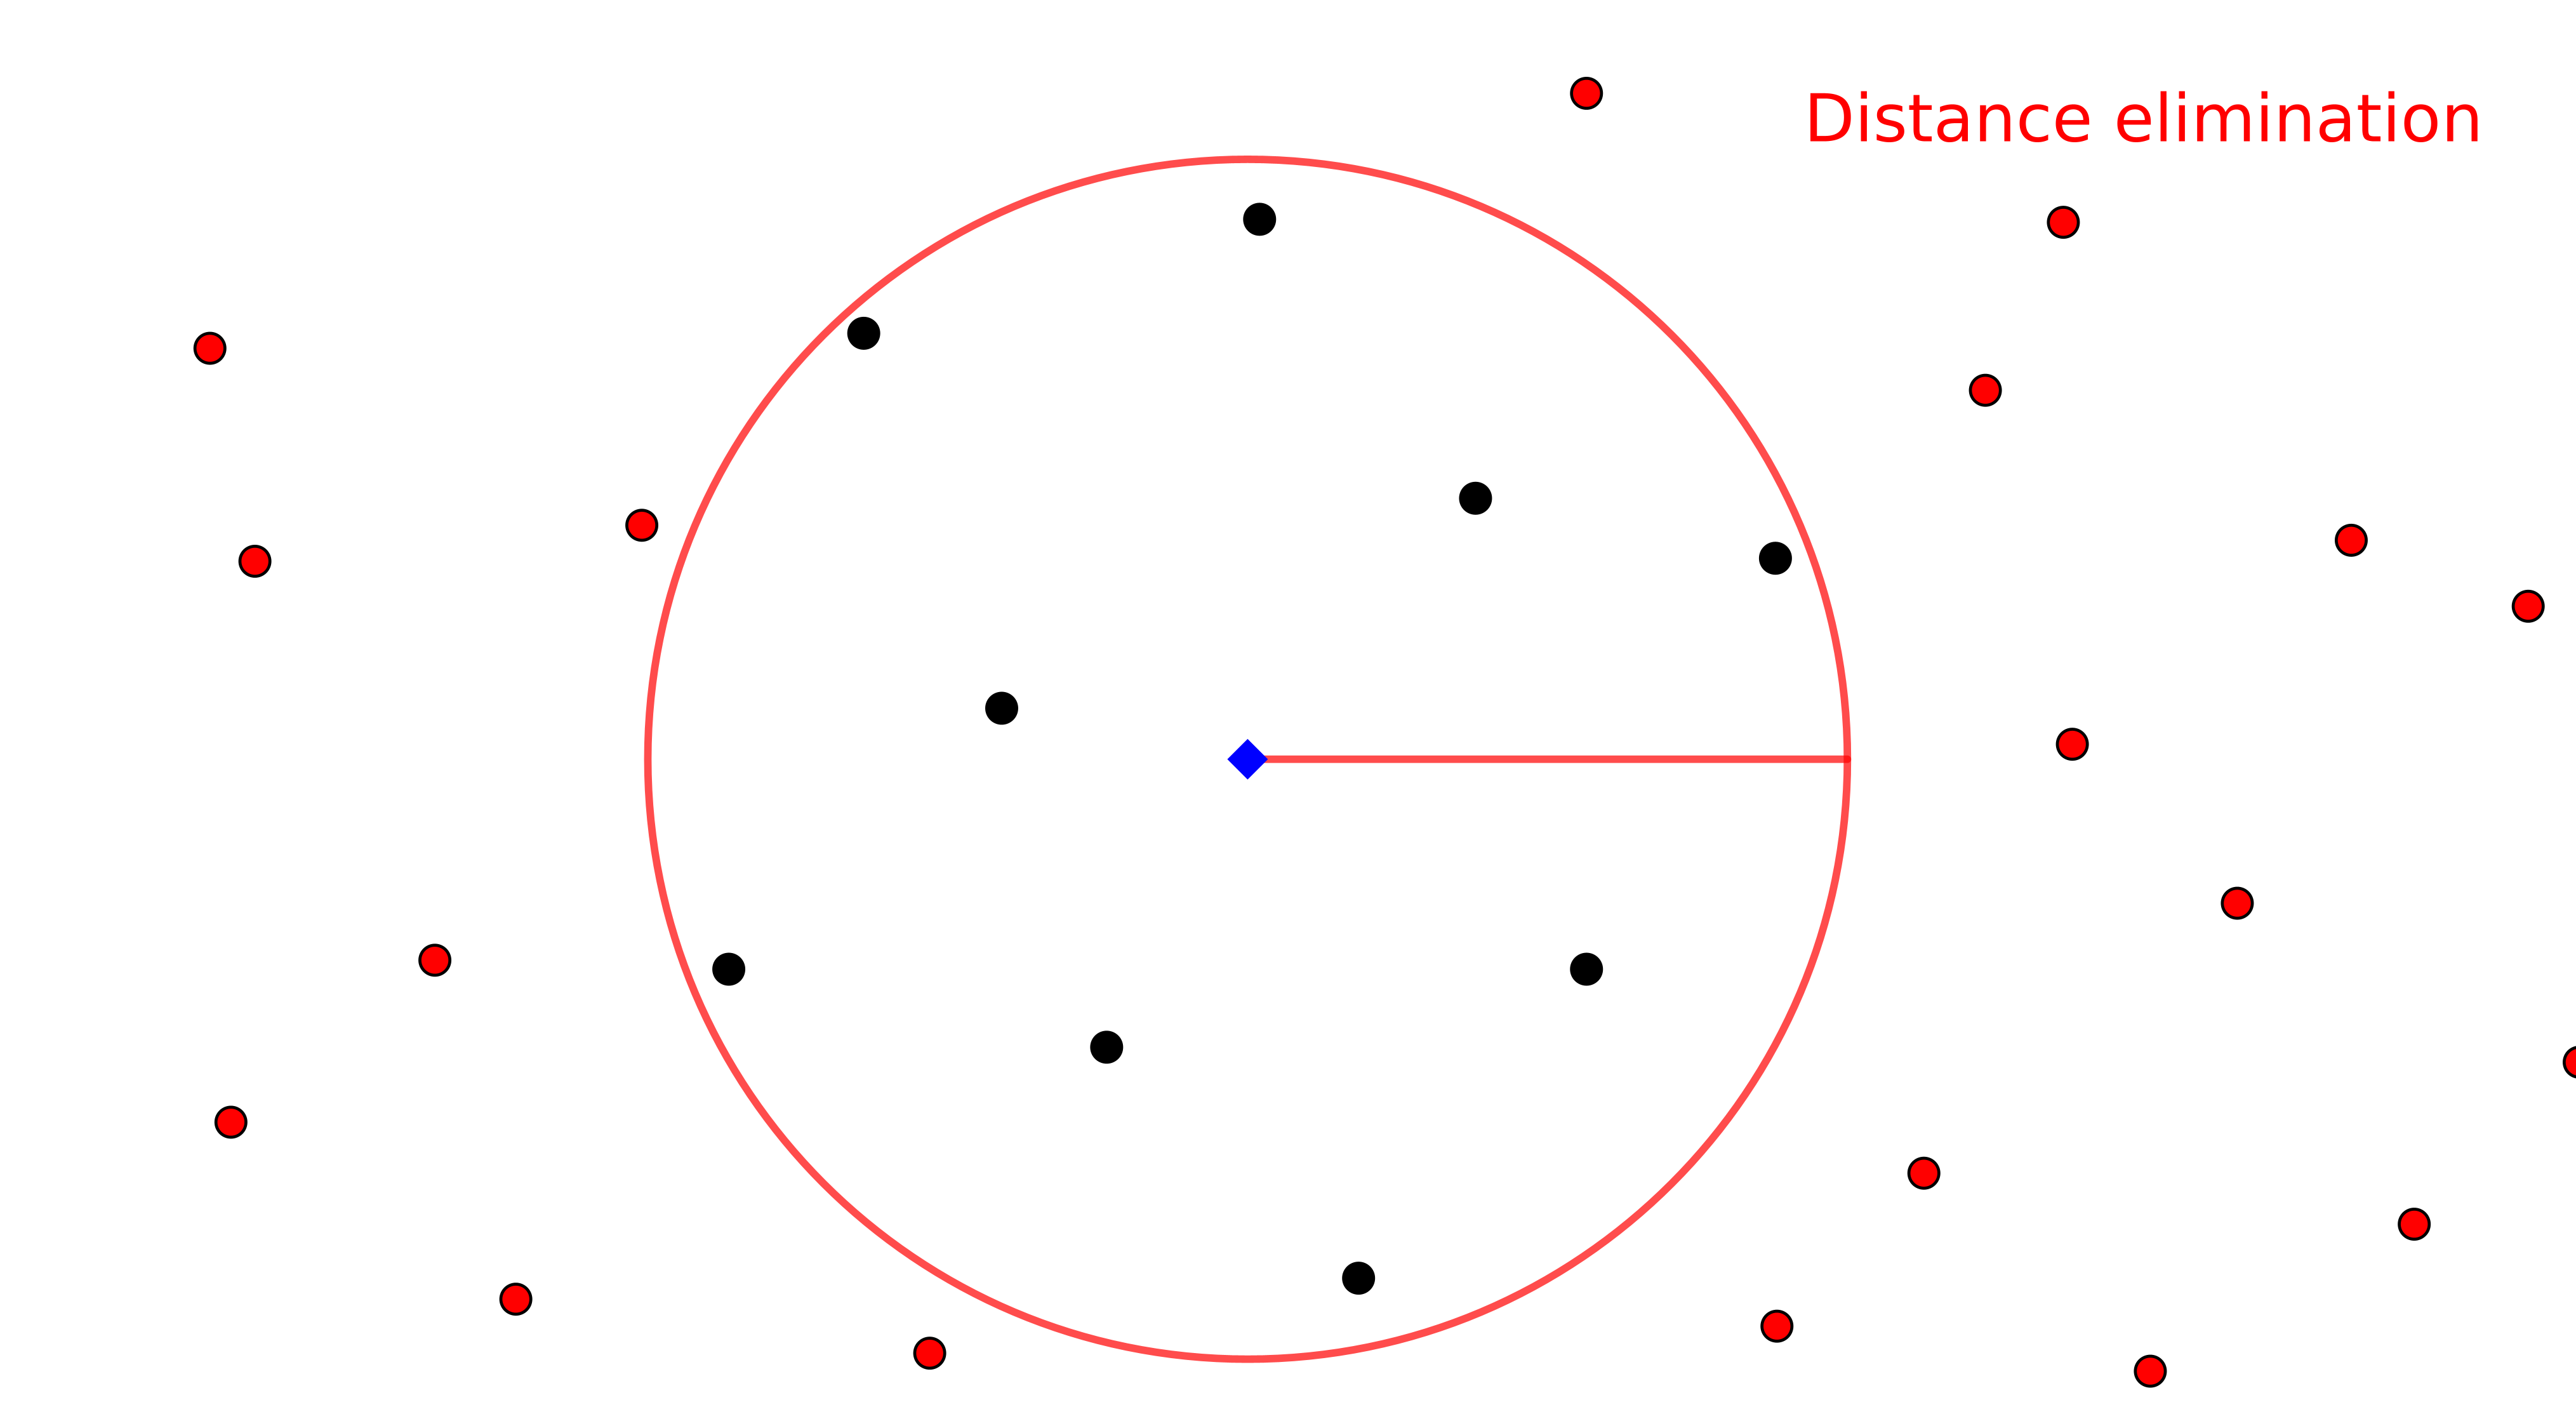
\includegraphics[width=2.5in]{images/illus_crit/distance_elim.png}}
    \caption{Example of a Delaunay triangulation}
    \label{fig:crit_dis}
\end{figure}

\begin{figure}[!t]
    \centering
    \boxed{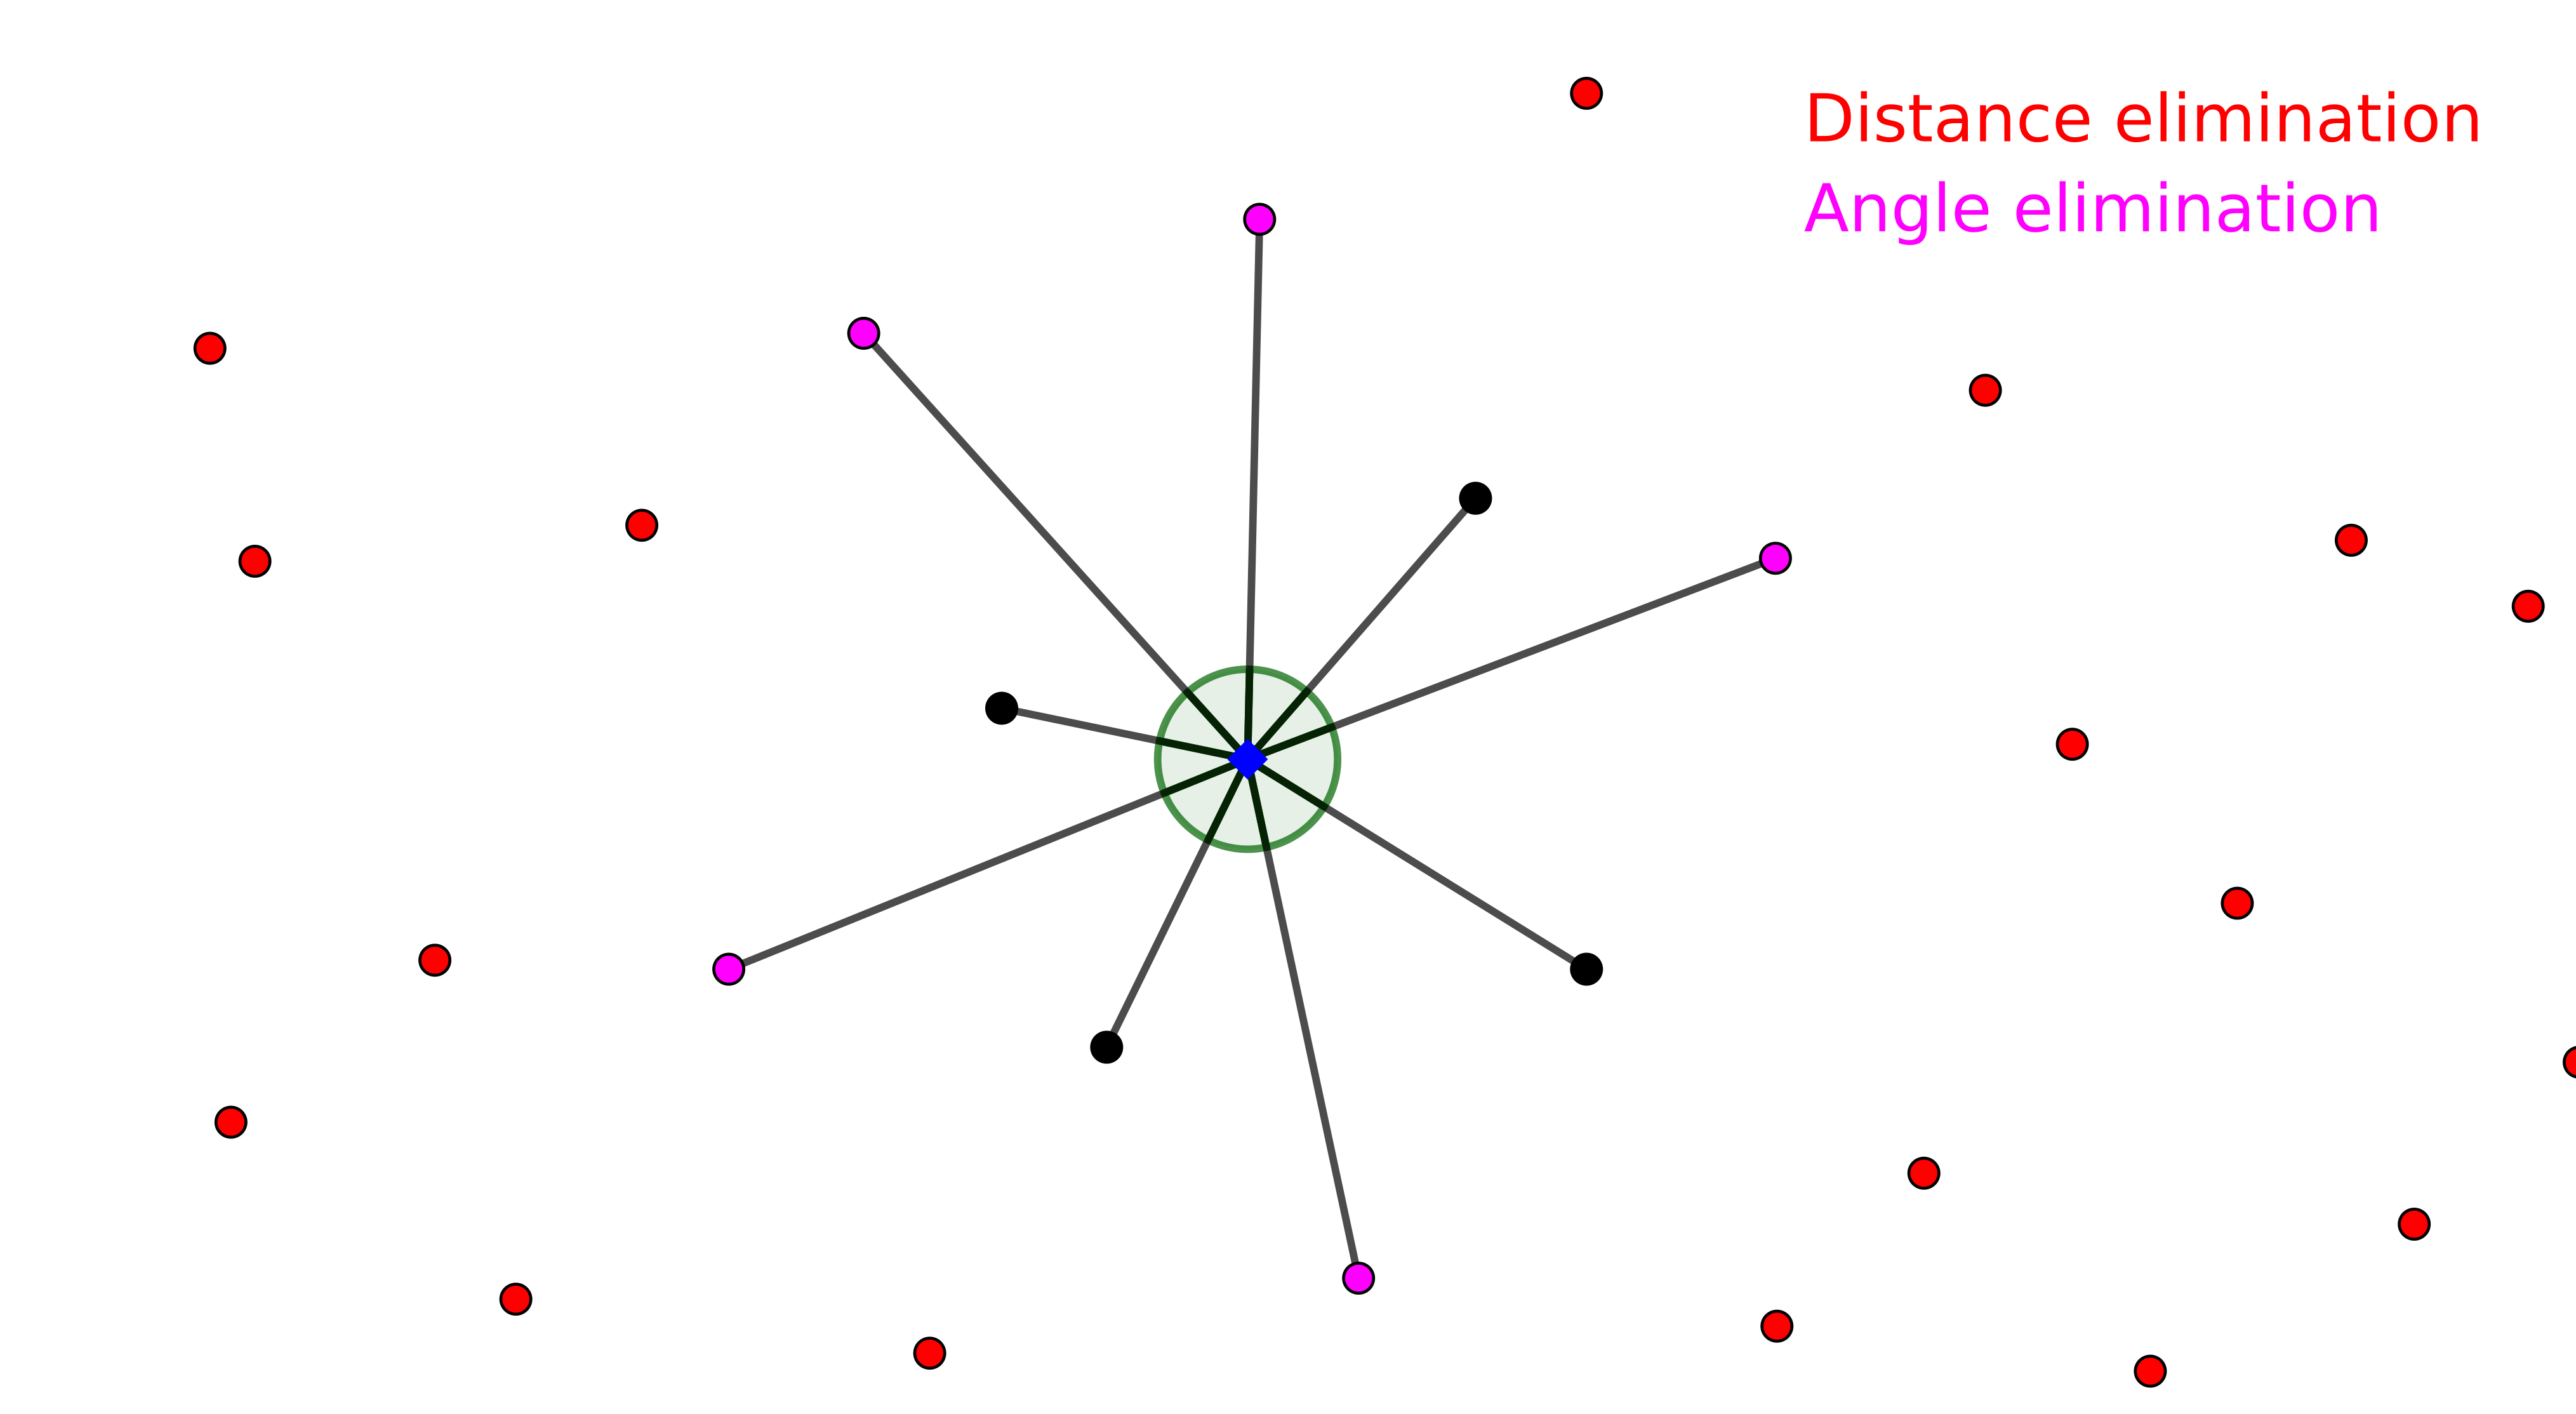
\includegraphics[width=2.5in]{images/illus_crit/angle_elim.png}}
    \caption{Example of a Delaunay triangulation}
    \label{fig:crit_ang}
\end{figure}

\begin{figure}[!b]
    \centering
    \boxed{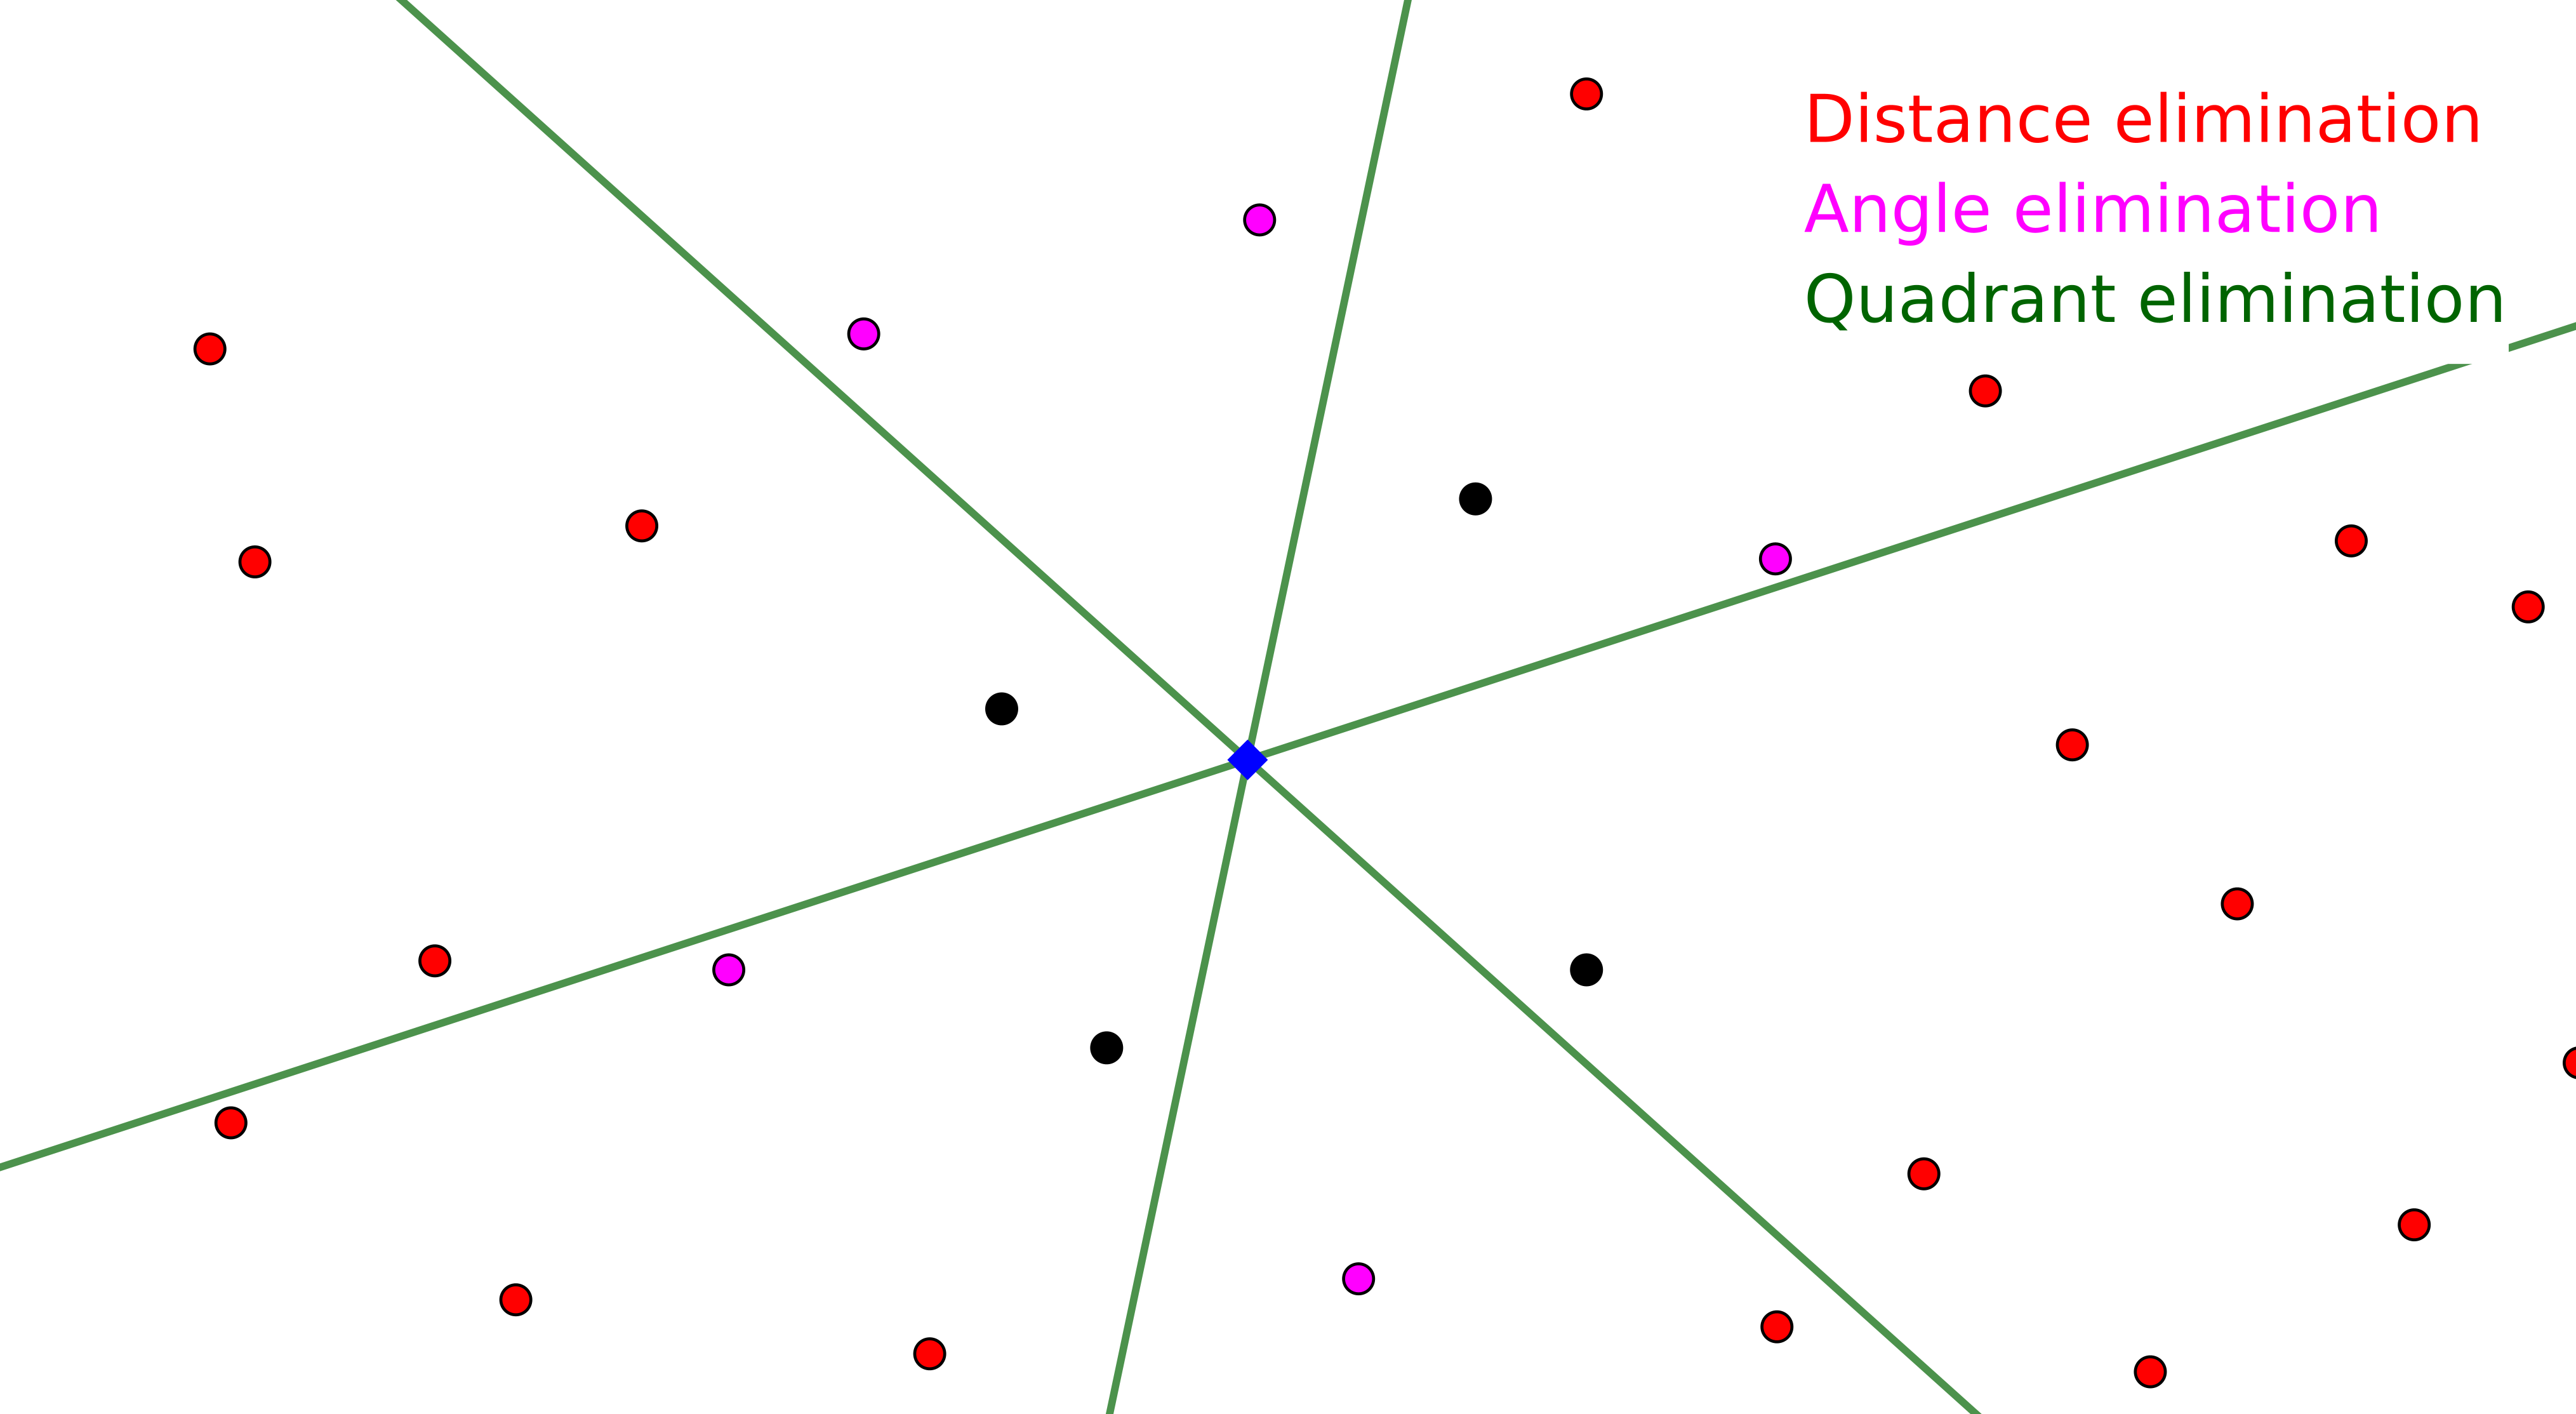
\includegraphics[width=2.5in]{images/illus_crit/quadrant_elim.png}}
    \caption{Example of a Delaunay triangulation}
    \label{fig:crit_qua}
\end{figure}

\begin{figure}[!t]
    \centering
    \boxed{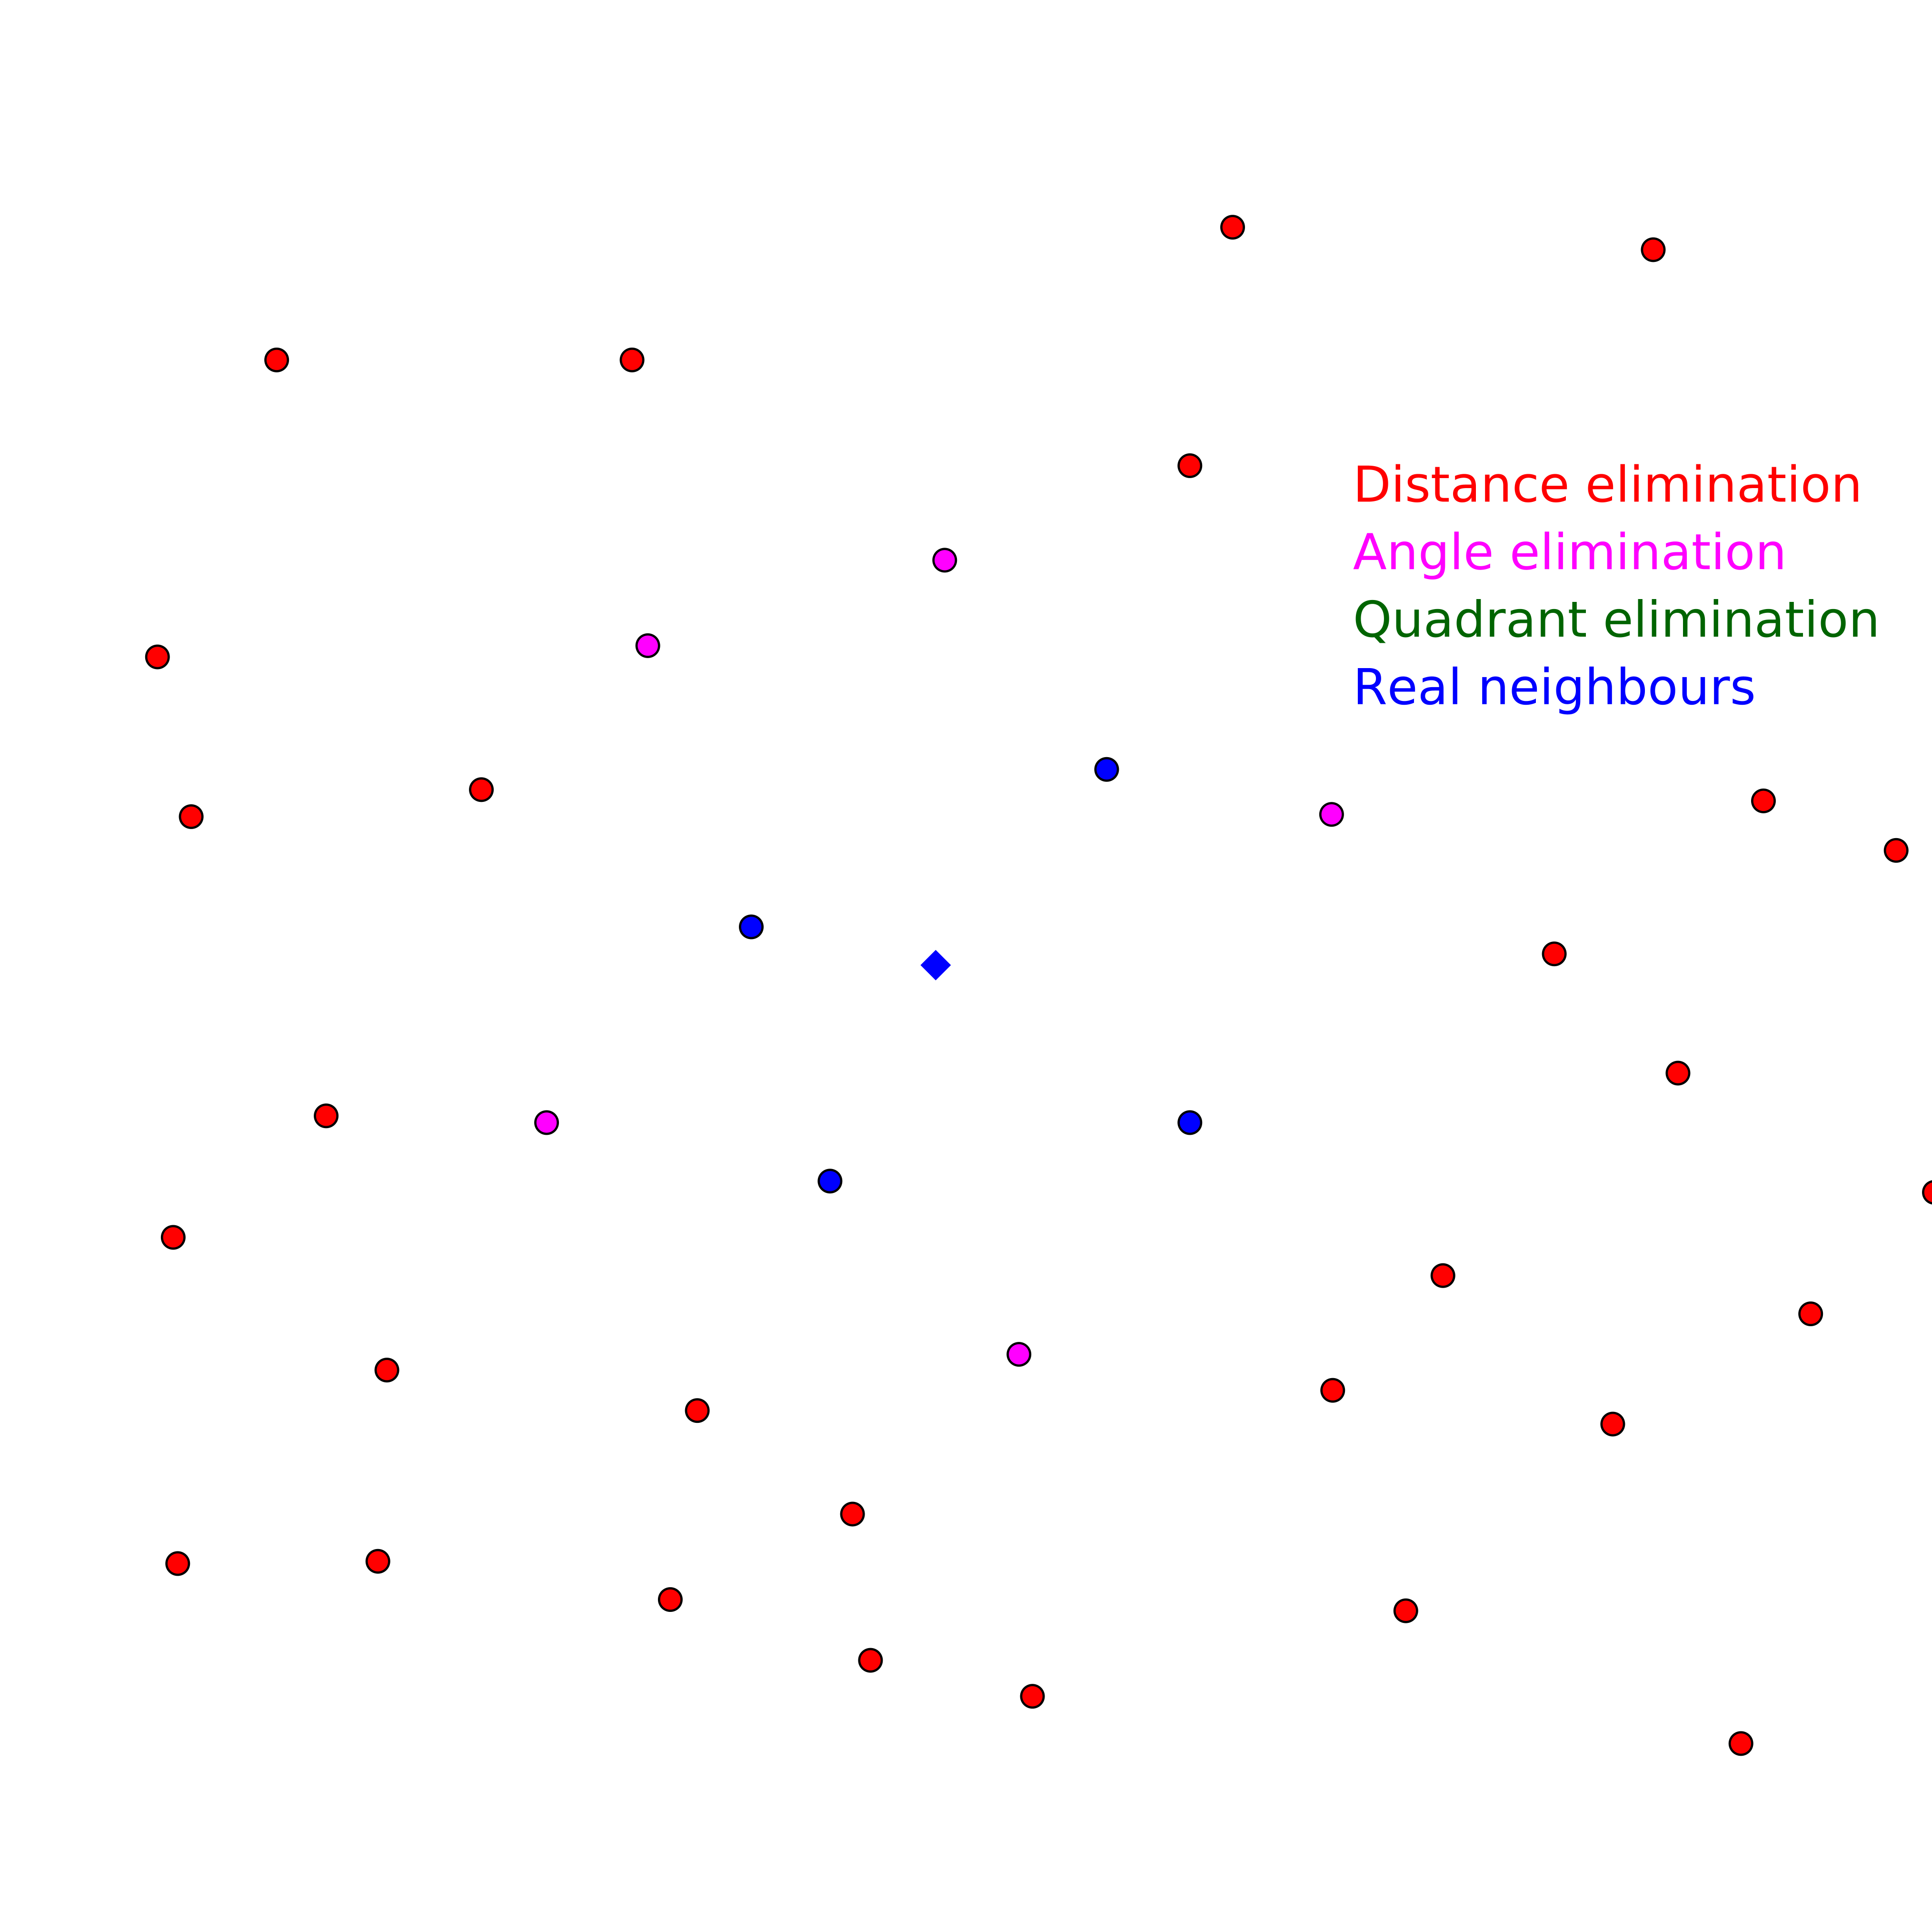
\includegraphics[width=2.5in]{images/illus_crit/neighs.png}}
    \caption{Example of a Delaunay triangulation}
    \label{fig:crit_nei}
\end{figure}

\subsubsection{Distance criterion}
When looking at the results of Delaunay triangulation, we realise that some edges, mostly on the border of $P$ are too long. Indeed, a \acrshort{bs} does not have an infinite coverage area.

As a consequence, for each \acrshort{bs} the neighbouring connexions that are longer than a certain value, called \emph{max\_distance}, are suppressed (cf. Table~\ref{table:crit_summary}).

\subsubsection{Angle criterion}
For each \acrshort{bs}, a potential neighbour can be \og hidden\fg{} by another one which nearer because there is a too narrow angle between those two \acrshort{bs}.
This criterion, will therefore suppress the longest edge between two \acrshort{bs} separated by a too small angle. This is illustrated in Figure~\ref{fig:crit_ang}.

\subsubsection{Quadrant criterion}
A version of this criterion, that was introduced here \cite{10201211} and used here \cite{art_del_paq}. Its goal is
to prevent all potential neighbours to be in the same angle range. Therefore, it was mainly thought to be used with the 
$k$-NN potential neigbours method.

It consists in dividing the space around each base station into quadrants and keeping only a certain number of potential neighbours
in each of the quadrants. The number of quadrants has been fixed to 6 (optimized here \cite{art_del_paq}).

The criterion has been upgraded by adding the possibility to rotate the quadrants. The offset angle selected, which is between 0 and 
60 degrees, is the one that maximises the sum of the distances of the potential neighbours to their closest quadrant delimitation.

In other words, it tends to select the angle with which the potential neighbors are as much in the middle of their respective quadrants
as possible.

The quadrant criterion is illustrated here Fig~\ref{fig:crit_qua}

\section{Results}

\subsection{Combining criteria}
As a matter of optimisation, criteria are applied one after another. For example, the base graph is Delaunay triangulation and we apply distance then angle.
The principle is that angle criterion will be applied on the Delaunay graph filtered with the distance criterion.

As a consequence, results differ according to the order in which the criteria are applied.

The best is Delaunay with distance and then angle.

\section{Conclusion}

[Ouverture : prendre en compte les zazimuths]

\printglossary[type=\acronymtype]
\printglossary

\bibliographystyle{IEEEtran}
\bibliography{./biblio.bib}

\end{document}


